\chapter*{ARE YOU A LIBERTARIAN?\\你是一个古典自由主义者吗}
\begin{paracol}{2}
\hbadness5000

Libertarianism starts with a simple statement of individual rights, but it raises hard questions. The fundamental political question is, do you make the decisions that are
important to your life, or does someone else make them for
you? Libertarians believe that individuals have both the right
and the responsibility to make their own decisions. Nonlibertarians of all political stripes believe that the government
should make some or many of the important decisions in an individual's life.
\switchcolumn
古典自由主义理论开始于一个对个人权利的陈述,但是它
提出了很艰深的问题。最基本的政治问题是,你生活中的重大
事务是你自己作决策,还是其他某些人替你作决策?古典自由
主义者相信个人有权利和责任自己作决策。所有政治光谱中的
非古典自由主义者都相信政府应当为个人生活中的某些或者很
多重要事务决定。
\switchcolumn*
For instance, consider whether you agree with the following:
\switchcolumn
例如,请思考一下你是否同意下面的观点:
\switchcolumn*
\begin{quotation}
\noindent As long as I respect the rights of others, I should have the
right to

Read whatever I want to---even if it offends others in the
community.

Choose the medical treatment I think is best---even if it's
risky.
\end{quotation}
\switchcolumn
\begin{quotation}
\noindent 只要我尊重其他人的权利,我就有权:

阅读我想阅读的任何东西 ---即使这些东西冒犯了社会中的其他人。

选择我认为最好的医疗方案 ---即使这可能很危险。
\end{quotation}
\switchcolumn*
If you answer yes to these questions, then you probably
agree with some basic libertarian positions on personal freedoms: the government has no business establishing a particular religion, enforcing moral codes, or regulating pornography
or hate speech. That doesn't mean libertarians endorse any of those particular choices, but it does mean they respect the
right of adults to make their own choices. Now consider some
other issues:
\switchcolumn
如果你对这些问题的回答是“是”,那么你也许赞同古典
自由主义关于个人自由的某些基本立场:政府不应设立某种形
式的国教、不应促进道德规则或者管制色情和表达仇恨的言
论。这并不是说古典自由主义者赞同任何上述观点和选择,但
这的确意味着他们尊重成年人做出自己选择的权利。现在请思
考以下的问题:
\switchcolumn*
\begin{quotation}
\noindent As long as I deal with others honestly, I should have the right to
	
	Earn more money than others even if I don't contribute money to charity.
	
	Leave my wealth to my children even though other children will be born with less.
\end{quotation}
\switchcolumn
\begin{quotation}
\noindent 只要我与其他人诚实相处,我就有权:

比其他人挣更多的钱,即使我不把钱捐给慈善事业。
	
把财富留给我的孩子,即使其他孩子出生的时候比我的孩子贫穷。
\end{quotation}
\switchcolumn*
If you answer yes to these questions, then you agree with the
basic libertarian goal of economic freedom. Now consider an-
other way of looking at freedom:
\switchcolumn
如果你对这些问题的回答是“是”,那么你就赞同古典自
由主义对经济自由的基本目标。现在我们用另外的方式来看一下自由:
\switchcolumn*
\begin{quote}
Should the government protect each individual's right to life,
liberty, and the pursuit of happiness, even though some people
will earn more than others, or use its power to try to make people more equal in monetary terms by transferring money from
some people to others?
\end{quote}
\switchcolumn
\begin{quote}
政府应当保护每个人的生命、财产和追求幸福的权利
吗,即使有人可能比其他人挣钱更多?或者政府应当运用
它的权力,通过将钱从一部分人手里转移到另一部分人手
里,让人们在货币分配的意义上更加平等吗?
\end{quote}
\switchcolumn*
If you are still in favor of freedom---as opposed to government coercion---to bring about a desired result, then you're
ready to measure your libertarianism.
\switchcolumn
如果你仍然希望自由带来你希望的结果,反对政府的强
制,那么你就已经准备好进行古典自由主义测试了。
\switchcolumn*
Again using the diamond chart described in chapter 1, we
now give you the opportunity to place yourself on the political
spectrum. In the modern American context, we frequently find
conservatives endorsing government restrictions on people's
personal choices, and liberals endorsing restrictions on their
economic decisions. Of course, that distinction is by no means
clear; conservatives may be more likely than liberals to favor
subsidies for big business, and many liberals support restrictions on smoking, gun ownership, and contributions to political
candidates.
\switchcolumn
现在我们再一次使用第一章中描述的菱形图,让你确定自
己在政治光谱上的坐标。在现代美国语境下,保守主义者常常
主张政府限制人们的个人选择,而自由派则限制人们的经济选
择。当然这种区分并不十分清晰;保守主义者也许比自由派更
倾向于资助大企业,而很多自由派也支持对吸烟、拥有枪支以
及政治献金进行限制。
\switchcolumn*
The following questionnaire asks whether you think it
should be your decision or the government's decision whether you engage in a variety of activities, which have been divided into
``Personal Freedoms'' and ``Economic Freedoms.'' (It should be
noted, however, that the division of individual choices into
``personal'' and ``economic'' is somewhat arbitrary. Every choice
involving your life is personal, and most choices involve property rights and economic exchange.)
\switchcolumn
后面的问题是问当参与各种活动时,你认为这些事务应当
由你自己决定还是由政府决定。这些问题划分为“个人自由”
和 “经济自由” (然而,需要注意的是,这种将个人选择划分
为 “个人事务” 和 “经济事务” 的方式有些武断。你生活当
中的每一次选择都是个人事务,而大多数选择都包含了财产权
和经济交换)。
\switchcolumn*
\textit{Give yourself 10 points if you think that you decide, 5 points if you're not sure,
and 0 points if you think the government decides. Then plot your score on the
diamond chart.}
\switchcolumn
\textbf{如果你非常确定应该由自己决定,请 给 打10分 ,如果不
确定,就打5分,如果你认为应该由政府来决定,就打0分。
然后将你的得分放在菱形图当中。}

\switchcolumn*[\section*{Personal Freedom\\个人自由}]
\begin{quotation}
\noindent Who should decide whether or not you

wear a seatbelt?

own a gun?

serve in the military?

smoke marijuana?

use a risky medical treatment?

engage in a homosexual relationship?

buy a pornographic video?

buy a sexist book?

send your child to a particular school?

have uncensored access to the Internet?
\end{quotation}

\noindent Total Personal Freedom score\rule[0pt]{2cm}{0.5pt}
\switchcolumn
\begin{quotation}
\noindent 应该由谁来决定你能否:

系安全带?

拥有枪支?

在军队服役?

抽大麻?

采用高风险的医疗方案?

和别人保持同性恋关系?

购买色情录像带?

购买色情书籍?

把你的孩子送到某个学校?

在没有审查的情况下上网?
\end{quotation}

\noindent 个人自由得分合计:\rule[0pt]{2cm}{0.5pt}

\switchcolumn*[\section*{Economic Freedom\\经济自由}]
\begin{quotation}
\noindent Who should decide whether or not you 

buy a foreign car?

put your retirement savings in Social Security?

give money to help the poor?

drive a taxicab without a license?

hire a worker of another race?

build a home without a permit?

pay subsidies to farmers?

work for less than minimum wage?

set up a mail-delivery company to compete with the Postal Service?

purchase flood or earthquake insurance?
\end{quotation}

\noindent Total Economic Freedom score\rule[0pt]{2cm}{0.5pt}
\switchcolumn
\begin{quotation}
\noindent 应该由谁来决定你能否:

购买外国车?

把你的退休储蓄放进社保系统?

捐钱来帮助穷人?

不需要执照就可以开出租车?

雇佣其他种族的员工?

不需要许可就可以建造房屋?

给农民补贴?

以低于最低工资的工资工作?

成立一家邮递公司与邮局竞争?

购买洪灾或地震保险?
\end{quotation}
\noindent 经济自由得分合计:\rule[0pt]{2cm}{0.5pt}
\switchcolumn*
Now plot your Personal Freedom score on the left scale of the
diamond chart and your Economic Freedom score on the right.
The intersection of your scores reveals your position on the political spectrum.
\switchcolumn
现在请把你的个人自由得分放在菱形图的左坐标轴上,把
你的经济自由得分放在右坐标轴上。你的得分的交叉点就表示
你在政治光谱中的位置。
\switchcolumn*
\begin{figure}[!htb]
	\centering
	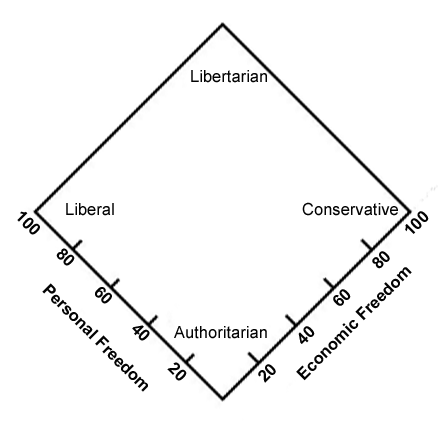
\includegraphics[width=0.7\linewidth]{1}
\end{figure}
\switchcolumn
\begin{figure}[!htb]
	\centering
	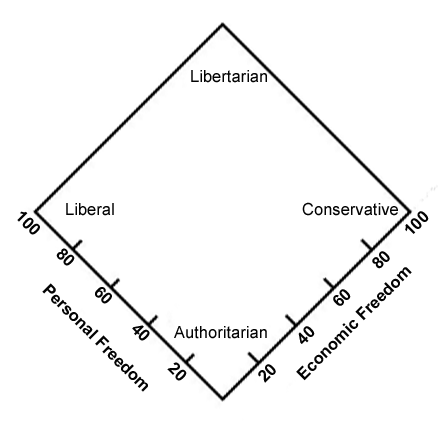
\includegraphics[width=0.7\linewidth]{1}
\end{figure}
\switchcolumn*
Very few people will have ``perfect'' scores in any direction. If
you've read this book, I hope that you've become convinced that
people can make most of the decisions about their lives better
than any legislator or regulator could and that you scored near
the top of the chart, in the Libertarian quadrant. (And if you
haven't read the book yet, I hope you'll do so and then take the
quiz again.) If so, welcome to the political movement that will
change the twenty-first century. If not, I hope you were at least
challenged and intrigued by the argument and that in the future
you'll notice more and more examples of the benefits of spontaneous order and the difficulties with coercive government.
\switchcolumn
在任何方向上都极少有人得“满分”。如果你已经读了这
本书,我希望你已经被说服,相信人们在大多数生活事务上自
己做决定,比任何议员或者管制官员做决定都要好。如果你的
得分几乎是在菱形图的顶端的话,那么你就已经是一个古典自
由主义者了(如果你还没读这本书,我希望你能够读完之后
再作一次测试)。如果是这样的话,欢迎你加入将会改变21世
纪的政治运动。如果不是的话,我希望你至少接受了本书论证
过程提出的挑战,或者至少本书引起了你的兴趣,而在将来,
你会看到越来越多的案例证明自发秩序所带来的好处以及强制
性政府所带来的困难。
\end{paracol}